\section{Parallel assets: the current multi-chain footprint and the case for consolidation}
\label{sec:parallel-assets}

A holder of \Flux is not necessarily holding anything on the \Flux main chain. Since early in the
project's life, tokens representing \flux have also been issued on other blockchains — a
``parallel asset'' is a token on a chain other than \Flux's own that is meant to track a \flux
balance, historically backed by reserves held at addresses the team controls rather than by a
supply-capped, on-chain-verifiable contract \srcroadmap{flux-roadmap-public.md:96}. Each such asset
adds a chain whose contract, custody keys, exchange relationships and accounting have to be kept in
sync with the main chain and with each other. This section inventories what actually exists today,
shows that the inventory has grown rather than shrunk even as the team has stated an intent to
consolidate it, describes the mechanism by which a parallel asset changes hands today and the trust
it requires, and states the settled but only partially resolved plan for reducing the footprint.
The bridging construction itself — mint-and-burn with attested proof-of-reserve — is specified in
\S\ref{sec:bridging}; this section establishes why that construction is needed and what it has to
replace.

\subsection{The inventory}
\label{sec:pa-inventory}

Table~\ref{tab:parallel-assets} lists every chain on which a \flux-denominated token is identified
by contract or account address in the surveyed code, together with the exact on-chain identifier
and its source. Ten entries are shipped by this definition: the address or module name appears in
code that a live, currently-operated service uses to read balances, construct transfers, or both.

\begin{table}[H]
\centering
\footnotesize
\caption{The parallel-asset footprint as read from the team's own indexing and swap tooling.
Ethereum, BNB Chain, Polygon and Avalanche C-Chain addresses agree between \texttt{holder-\allowbreak{}snapshot}
and \texttt{flux-\allowbreak{}supply-\allowbreak{}tracker}; Base appears only in the latter. \shipped for every row —
each identifier is consumed by code that treats it as a live contract or account, not asserted from
a roadmap or design note. None of these addresses was independently verified against the chain
itself by the evidence gathering this section relies on.}
\label{tab:parallel-assets}
\begin{tabular}{@{}llp{6.1cm}l@{}}
\toprule
Asset & Chain & Contract / account identifier & Provenance \\
\midrule
FLUX (ERC-20) & Ethereum &
\texttt{\scriptsize 0x720cd16b\allowbreak{}011b987d\allowbreak{}a3518fbf\allowbreak{}38c3071d\allowbreak{}4f0d1495} &
\srccode{holder-snapshot/\allowbreak{}index.js}{22}\srccode{flux-supply-tracker/\allowbreak{}index.html}{310} \\
FLUX (BEP-20) & BNB Chain &
\texttt{\scriptsize 0xaff9084f\allowbreak{}23745858\allowbreak{}79e8b434\allowbreak{}c399e29e\allowbreak{}80cce635} &
\srccode{holder-snapshot/\allowbreak{}index.js}{23}\srccode{flux-supply-tracker/\allowbreak{}index.html}{319} \\
FLUX (ERC-20-compatible) & Polygon &
\texttt{\scriptsize 0x\allowbreak{}A2bb7A68\allowbreak{}c46b53f6\allowbreak{}Bb\allowbreak{}F6c\allowbreak{}C91\allowbreak{}C865Ae24\allowbreak{}7A82E99B} &
\srccode{holder-snapshot/\allowbreak{}index.js}{26}\srccode{flux-supply-tracker/\allowbreak{}index.html}{328} \\
FLUX (ERC-20-compatible) & Avalanche C-Chain &
\texttt{\scriptsize 0xc4B06F17\allowbreak{}ECc\allowbreak{}B2215\allowbreak{}a5DBf042\allowbreak{}C672101F\allowbreak{}c20da\allowbreak{}F55} &
\srccode{holder-snapshot/\allowbreak{}index.js}{24}\srccode{flux-supply-tracker/\allowbreak{}index.html}{337} \\
FLUX (ERC-20-compatible) & Base &
\texttt{\scriptsize 0xb008bdcf\allowbreak{}9cdff9da\allowbreak{}684a1909\allowbreak{}41dc3dca\allowbreak{}8c2cdd44} &
\srccode{flux-supply-tracker/\allowbreak{}index.html}{346} (absent from \texttt{holder-\allowbreak{}snapshot}) \\
FLUX (SPL mint) & Solana &
\texttt{\scriptsize FLUX1wa2\allowbreak{}Gmbt\allowbreak{}SB6Z\allowbreak{}Gi2p\allowbreak{}TNb\allowbreak{}V\allowbreak{}Cw3z\allowbreak{}Ee\allowbreak{}Kn\allowbreak{}a\allowbreak{}PCk\allowbreak{}Pt\allowbreak{}FX\allowbreak{}xq\allowbreak{}Xe} &
\srccode{holder-snapshot/\allowbreak{}index.js}{20}\srccode{flux-supply-tracker/\allowbreak{}index.html}{355} \\
FLUX (ASA) & Algorand &
\texttt{\scriptsize 1029804829} &
\srccode{holder-snapshot/\allowbreak{}index.js}{27}\srccode{flux-supply-tracker/\allowbreak{}index.html}{364} \\
FLUX (Ergo token) & Ergo &
\texttt{\scriptsize e8b20745\allowbreak{}ee9d1881\allowbreak{}7305f32e\allowbreak{}b2101583\allowbreak{}1a48f02d\allowbreak{}40980de6\allowbreak{}e849f886\allowbreak{}dca7f807} &
\srccode{holder-snapshot/\allowbreak{}index.js}{25}\srccode{flux-supply-tracker/\allowbreak{}index.html}{373} \\
FLUX (TRC-20) & Tron &
\texttt{\scriptsize TWr6yzuk\allowbreak{}Rw\allowbreak{}Z53HDe\allowbreak{}3bzc\allowbreak{}C8RC\allowbreak{}Tbi\allowbreak{}Ka4Zz\allowbreak{}b6} &
\srccode{holder-snapshot/\allowbreak{}index.js}{21}\srccode{flux-supply-tracker/\allowbreak{}index.html}{382} \\
FLUX (Pact fungible-v2) & Kadena &
\texttt{\scriptsize runonflux.\allowbreak{}flux} &
\srccode{flux-kda/\allowbreak{}flux.pact}{1-3}\srccode{flux-supply-tracker/\allowbreak{}index.html}{391} \\
\bottomrule
\end{tabular}
\end{table}

The EVM entries (Ethereum, BNB Chain, Polygon, Avalanche C-Chain, Base) are read via each chain's
ERC-20 \texttt{Transfer} log topic by the same crawler code
\shipped \srccode{holder-snapshot/\allowbreak{}eth.js}{63-88}, so they are one contract shape deployed five
times rather than five independent designs; the Ethereum/BNB-Chain pair is additionally attested by
its own source repository as the same compiled bytecode on both chains
\srcdoc{flux-eth-bsc/README.md:1-14}. That repository's own Truffle build record, however,
contains no deployed network address for any chain — the \texttt{networks} field of
\texttt{flux-eth-bsc/\allowbreak{}bin/\allowbreak{}Flux.\allowbreak{}json} is absent or empty \srcdoc{flux-eth-bsc/bin/Flux.json,
\texttt{networks} field}. Every address in Table~\ref{tab:parallel-assets} is taken
from the team's own indexing tools, not from the contract-source repository itself.

\subsection{The trend is the wrong way}
\label{sec:pa-trend}

Three snapshots of the team's own tooling, taken at different times, give three different chain
counts, and the count only goes up. \texttt{holder-\allowbreak{}snapshot}'s \texttt{README} documents support
for six chains \srcdoc{holder-snapshot/README.md:4-10}; its own \texttt{index.js} code
handles eight, adding Polygon and Algorand beyond what the README claims
\shipped \srccode{holder-snapshot/\allowbreak{}index.js}{20-27}; and \texttt{flux-\allowbreak{}supply-\allowbreak{}tracker}'s live
\texttt{CHAINS} configuration, last touched 2026-08-05, carries ten, adding Base and folding Kadena
in as a tenth \shipped \srccode{flux-supply-tracker/\allowbreak{}index.html}{308-397}. Read plainly: documentation
said six, shipped code already did eight, and the newest measurement tool does ten. This is the
team's own data, gathered to run its own reserve and rich-list computations, and it is the single
strongest argument in this section for consolidation — not because any one parallel asset is
individually a problem, but because the footprint has been growing under a team that has also, in
the same period, stated a public non-goal of not adding new parallel-asset chains while the existing
ones are consolidated \srcroadmap{flux-roadmap-public.md:209}. The growth already happened before
that statement was made, which is exactly why consolidation is a live problem and not a preventative
one.

\begin{figure}[H]
\centering
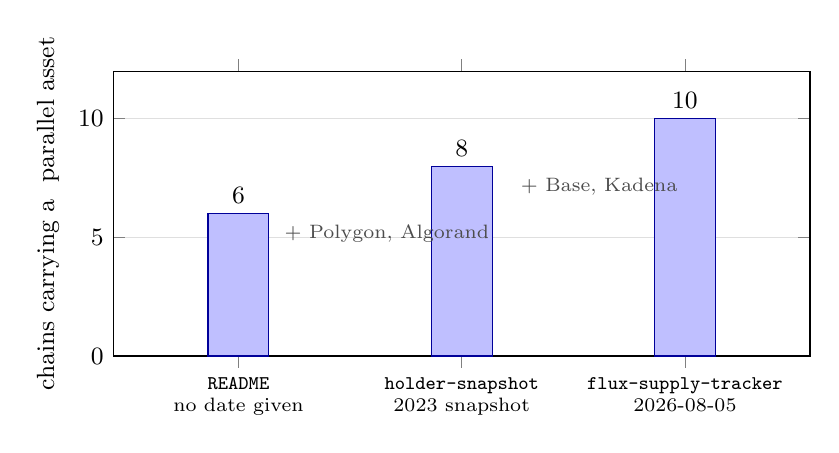
\begin{tikzpicture}[font=\small]
\begin{axis}[
  width=0.86\linewidth, height=5.2cm,
  ybar, bar width=22pt,
  ymin=0, ymax=12,
  ylabel={chains carrying a \flux{} parallel asset},
  symbolic x coords={README, snapshot, tracker},
  xtick=data,
  xticklabels={%
    {\texttt{README}\\{\scriptsize no date given}},
    {\texttt{holder-\allowbreak{}snapshot}\\{\scriptsize 2023 snapshot}},
    {\texttt{flux-\allowbreak{}supply-\allowbreak{}tracker}\\{\scriptsize 2026-08-05}}},
  xticklabel style={align=center, font=\scriptsize},
  nodes near coords, nodes near coords style={font=\small\bfseries},
  ymajorgrids, major grid style={gray!25},
  enlarge x limits=0.28,
]
\addplot[fill=blue!25, draw=blue!60!black] coordinates {(README,6) (snapshot,8) (tracker,10)};
\end{axis}
\node[anchor=west, font=\scriptsize, text=black!70] at (2.05,1.55) {$+$ Polygon, Algorand};
\node[anchor=west, font=\scriptsize, text=black!70] at (5.05,2.15) {$+$ Base, Kadena};
\end{tikzpicture}
\caption{The parallel-asset footprint grew between every source that documents it, and no single
source is current. The count is six in the repository README, eight in the \texttt{holder-\allowbreak{}snapshot}
code path, and ten in \texttt{flux-\allowbreak{}supply-\allowbreak{}tracker}; the two chains added at each step are annotated.
This is the measurement problem \S\ref{sec:pa-supply-accounting} addresses: a consolidation cannot be
scoped from a source that does not know how many chains exist. \shipped
\srcdoc{holder-snapshot/README.md:4-10}\srccode{holder-snapshot/\allowbreak{}index.js}{20--27}\srccode{flux-supply-tracker/\allowbreak{}index.html}{308--397}.}
\label{fig:pa-chain-growth}
\end{figure}

One further caveat belongs here rather than in a footnote: as of the most recent local state of
\texttt{holder-\allowbreak{}snapshot}, only its Ergo crawl is actually invoked — every other chain's
\texttt{start()} call is commented out \shipped \srccode{holder-snapshot/\allowbreak{}index.js}{29-36} — so the
tool that produced the ten-chain figure is not itself being run against ten chains today. That
does not change the ten-chain count in the newer tracker, which is the operative figure.

\subsection{How a parallel asset is acquired today}
\label{sec:pa-acquisition}

Two mechanisms exist for turning a claim on one chain into a balance on another, and both are
mediated by the same custodial system, \Fusion (\texttt{Zel\allowbreak{}Core-\allowbreak{}io/\allowbreak{}fusion}), an Express service the
team operates at \texttt{fusion.\allowbreak{}runonflux.\allowbreak{}io}
\shipped \srccode{fusion/\allowbreak{}config/\allowbreak{}default.js}{6}, \srccode{fluxswap/\allowbreak{}lib/\allowbreak{}api/\allowbreak{}services/\allowbreak{}swap\_service.dart}{10}.

\textbf{Cross-chain swap.} A holder deposits to a \Fusion-controlled address on the source chain
(one of eleven \texttt{swapsecrets} addresses, one per chain --- the main chain and the ten parallel chains ---
\shipped \srccode{fusion/\allowbreak{}config/\allowbreak{}default.js}{434-482}); \Fusion's automation loop detects the
deposit \shipped \srccode{fusion/\allowbreak{}src/\allowbreak{}services/\allowbreak{}swapAutomationService.js}{736-800}, and once
confirmation thresholds are met, its resolver signs and broadcasts the equivalent send on the
destination chain from that chain's own single hot-wallet key
\shipped \srccode{fusion/\allowbreak{}src/\allowbreak{}services/\allowbreak{}swapService.js}{997-1006}. Nothing is signed by the holder in
this path beyond the original deposit transaction.

\textbf{Snapshot claim.} For balances established by an earlier, offline snapshot (an operator runs
\texttt{flux-\allowbreak{}cli printsnapshot} and the resulting balances are loaded into \Fusion's database
\srcdoc{fusion/README.md:29}), the holder proves ownership by signing a
server-issued, single-use message phrase with the private key of the recorded source address
\shipped \srccode{fusion/\allowbreak{}src/\allowbreak{}services/\allowbreak{}claimSnapshotService.js}{202-207}. \Fusion verifies that
signature against the recorded address using a chain-specific signature-validation routine
\shipped \srccode{fusion/\allowbreak{}src/\allowbreak{}services/\allowbreak{}generalService.js}{349-563}, then pays out the claimed amount
from the same per-chain custodial hot wallet used for swaps
\shipped \srccode{fusion/\allowbreak{}src/\allowbreak{}services/\allowbreak{}claimSnapshotService.js}{250-286}.

In both paths, the trust assumption is the same at the point of payout: a single private key per
chain per role, held by the \Fusion operator, with no multisig, threshold signature, or on-chain
escrow gating the outbound send \shipped \srccode{fusion/\allowbreak{}src/\allowbreak{}coinLibs/\allowbreak{}eth.js}{66-101}. What a holder
signs proves ownership of a source-chain balance; it authorizes nothing about the destination-chain
payment, which is entirely at the operator's discretion once the claim is validated.

\textbf{Kadena is a distinct, additional case.} Kadena-denominated \flux increases only through the
Pact module's \texttt{fund} function, which is gated by a 2-of-3 multisig keyset held by the team
\shipped \srccode{flux-kda/\allowbreak{}flux.pact}{12-14,84-89}, \srccode{flux-kda/\allowbreak{}env}{2--9}. Eligibility for a Kadena node-reward payout is
computed off-chain: a node self-reports its status
\shipped \srccode{fluxstats/\allowbreak{}src/\allowbreak{}services/\allowbreak{}kadenaService.js}{119}, a team-run crawler polls that
status every two hours \shipped \srccode{fluxstats/\allowbreak{}src/\allowbreak{}services/\allowbreak{}kadenaService.js}{171-173}, and
nothing in the Pact contract itself constrains what a \texttt{fund} call may credit or on what basis
\shipped \srccode{flux-kda/\allowbreak{}flux.pact}{84-89}. The claim path that converts an eligibility figure into a credited balance
does exist, and it was located outside the repositories this section first examined. A holder proves
ownership of a main-chain address by signing a one-time server-issued phrase, verified against the
legacy Zelcash signature scheme \shipped \srccode{fusion/\allowbreak{}src/\allowbreak{}services/\allowbreak{}generalService.js}{378-390}.
Eligibility is then computed by \Fusion's backend from its own private index of \Flux daemon coinbase
transactions, at a flat 10\% per chain
\shipped \srccode{fusion/\allowbreak{}src/\allowbreak{}services/\allowbreak{}coinbaseService.js}{6-25,103-157}. Payout is not a mint: it is a
plain Pact \texttt{transfer} from a team treasury account, signed by a single team-held hot key
\shipped \srccode{fusion/\allowbreak{}src/\allowbreak{}coinLibs/\allowbreak{}kda.js}{231-300}, \srccode{fusion/\allowbreak{}config/\allowbreak{}default.js}{393-395}.

So the \texttt{fund} capability and the claim path are two separate mechanisms, and the claim path
never invokes the mint. Every step is team-mediated: a team-run database decides eligibility, a single
team-held key executes the payout, and the 2-of-3 team keyset alone can increase supply. The only step
not under team control is the holder's initial signature proving address ownership. What remains
undocumented in any surveyed repository is how and when the treasury account is replenished through
that 2-of-3 mint --- which is the one place where Kadena-denominated supply actually grows. The
repository named for this mechanism, \texttt{kadena-\allowbreak{}distribution-\allowbreak{}public}, still contains only a licence
and a two-line README \srcdoc{kadena-distribution-public/README.md:1-2}.

\subsection{The supply-accounting problem}
\label{sec:pa-supply-accounting}

Any published figure for how much \flux is in circulation, net of parallel-asset reserves the team
itself holds, depends on a list of which addresses count as ``team reserve.'' Three such lists exist
in the surveyed corpus, and only one of them is authoritative: \texttt{balance-\allowbreak{}checker}
(\texttt{RunOnFlux/\allowbreak{}balance-checker}), the repository the team itself runs to monitor its own
issuer-controlled addresses \shipped \srccode{balance-checker/\allowbreak{}config/\allowbreak{}default.js}{39-232} --- not
\texttt{fluxstats} and not \texttt{flux-\allowbreak{}supply-\allowbreak{}tracker}. \texttt{flux-\allowbreak{}supply-\allowbreak{}tracker}'s own source
comment corroborates this: it states that its locked-reserve figures come ``from the public Fusion
balance checker (github.com/RunOnFlux/balance-checker), which monitors the same set''
\shipped \srccode{flux-supply-tracker/\allowbreak{}index.html}{301--303}.

On Ethereum, \texttt{fluxstats}'s rich-list service excludes twelve addresses
\shipped \srccode{fluxstats/\allowbreak{}src/\allowbreak{}services/\allowbreak{}richListService.js}{146-153}, while
\texttt{flux-\allowbreak{}supply-\allowbreak{}tracker}'s reserve-wallet configuration for the same chain excludes seven
\shipped \srccode{flux-supply-tracker/\allowbreak{}index.html}{311-317}. An earlier reading of this gap in the
paper treated it as a genuine disagreement over what counts as reserve. \textbf{That reading is
superseded.} The root cause is known and it is benign: \texttt{fluxstats}'s Ethereum exclude list
still names the ETH \texttt{LOCKED} address as it stood before an August 2026 key rotation,
\texttt{0xa23702e9349fbf\allowbreak{}9939864da1245f5b\allowbreak{}358e7ef30b}, rather than the current address,
\texttt{0x3d1759846bbbde\allowbreak{}b7f71558d1fc6f00\allowbreak{}916006a795}
\shipped \srccode{fluxstats/\allowbreak{}src/\allowbreak{}services/\allowbreak{}richListService.js}{152}
\srccode{balance-checker/\allowbreak{}config/\allowbreak{}default.js}{98}. The same stale-rotation lag, not a deeper
disagreement, also accounts for \texttt{fluxstats}'s BSC \texttt{LOCKED} entry
\shipped \srccode{fluxstats/\allowbreak{}src/\allowbreak{}services/\allowbreak{}richListService.js}{171} and its \Flux main-chain
\texttt{COLD} entry \shipped \srccode{fluxstats/\allowbreak{}src/\allowbreak{}services/\allowbreak{}richListService.js}{74}, both of which
still name the address each replaced. Neither tool was conceptually wrong about what counts as a
reserve address; one was simply not updated when the addresses it tracks rotated.

Of the two addresses an earlier draft of this section left as disputed: \texttt{0x3d1759846bbbde\allowbreak{}b7f71558d1fc6f00\allowbreak{}916006a795}
is confirmed issuer-held --- it is \texttt{balance-\allowbreak{}checker}'s own current ETH \texttt{LOCKED} address
\shipped \srccode{balance-checker/\allowbreak{}config/\allowbreak{}default.js}{98} and holds \num{279000000}\flux
\shipped \srcmeasured{ethereum-rpc.publicnode.com}{2026-09-03}.
\texttt{0x9b77c6af70878c\allowbreak{}5c748d0ab456dcac\allowbreak{}1dfc01f962} (labelled ``fees'' in
\texttt{flux-\allowbreak{}supply-\allowbreak{}tracker} only) is absent from the authoritative registry on every chain and
holds zero on every EVM chain queried; it is dropped from this accounting
\shipped \srcmeasured{public RPC, per-chain endpoints}{2026-09-03}.

\paragraph{\texttt{totalSupply} is not the outstanding liability.} Every EVM parallel asset was
minted at the full nominal \num{440000000}\flux at contract construction: Ethereum, BNB Chain,
Avalanche C-Chain and Base each report a \texttt{totalSupply} of exactly \num{440000000}\flux, as do
the Algorand ASA and the Ergo token; the Solana mint reports \num{59999990.375}\flux
\shipped \srcmeasured{public RPC, per-chain endpoints}{2026-09-03}. \num{440000000} is also
\maxmoney in \fluxd, a per-transaction sanity bound rather than a supply cap
\srcroadmap{flux-roadmap-public.md:189,191} (\Cref{sec:monetary-policy}). Eight of the ten chains
(Table~\ref{tab:issuer-liability}) each holding
the entire nominal cap, against a main chain that has issued \num{429466823.97}\flux in total
(\Cref{sec:monetary-policy}), makes the point on its own: \texttt{totalSupply} measures what was
minted into a contract, not what remains outstanding. What becomes of the issuer-held remainder is
decided: the Foundation immobilises its own legacy holdings by transferring them to a published
per-chain dead address (\S\ref{sec:bridging-migration}; \planned
\srcintent{design intake}).

\paragraph{Measured outstanding liability, all ten chains resolved.} Using \texttt{balance-\allowbreak{}checker}'s
registry as the operand, the outstanding liability --- \texttt{totalSupply} minus the sum of the six
current, post-rotation issuer addresses per chain (\texttt{SNAPSHOT}, \texttt{MINING},
\texttt{SWAP}, \texttt{LOCKED}, \texttt{LOCKED SNAPSHOT}, \texttt{LOCKED MINING}) --- is now measured
for all ten legacy assets. Retrieved
2026-09-03T11:23:06Z (Ethereum, BNB Chain, Avalanche C-Chain, Base) and 2026-09-04 (Solana, Algorand, Polygon, Ergo, Tron, Kadena); reproducible
with \texttt{scripts/\allowbreak{}13-issuer-balances.\allowbreak{}sh}, \texttt{scripts/\allowbreak{}15-nonevm-liability.\allowbreak{}sh} and
\texttt{scripts/\allowbreak{}16-remaining-liability.\allowbreak{}sh},
\texttt{scripts/\allowbreak{}18-tron-final.\allowbreak{}sh} and \texttt{scripts/\allowbreak{}19-kadena-ledger.\allowbreak{}js}.

\begin{table}[H]
\centering\footnotesize
\caption{Outstanding parallel-asset liability by chain, using \texttt{balance-\allowbreak{}checker}'s registry of
issuer-controlled addresses as the operand. All ten legacy assets are measured from key-free public
endpoints. Nominal supply differs by chain: the eight EVM-style deployments were each minted at
\num{440000000}, Solana at \num{59999990.375}, and Kadena at \num{39998820.81}.
\shipped \srcmeasured{scripts/\allowbreak{}13-issuer-balances.sh}{2026-09-03};
\srcmeasured{scripts/\allowbreak{}15-nonevm-liability.sh, scripts/\allowbreak{}16-remaining-liability.sh,
scripts/\allowbreak{}18-tron-final.sh, scripts/\allowbreak{}19-kadena-ledger.js, scripts/\allowbreak{}20-kadena-issuer.js}{2026-09-04}.}
\label{tab:issuer-liability}
\begin{tabular}{@{}lrrr@{}}
\toprule
Chain & \texttt{totalSupply} (\flux) & Issuer-held (\flux) & Outstanding (\flux) \\
\midrule
\multicolumn{4}{@{}l}{\itshape Surviving --- snapshot-carried, no holder action} \\
Ethereum & \num{440000000.00000000} & \num{283782657.21951687} & \textbf{\num{156217342.78048313}} \\
BNB Chain & \num{440000000.00000000} & \num{379416462.37025207} & \textbf{\num{60583537.62974790}} \\
\addlinespace
\multicolumn{4}{@{}l}{\itshape Retiring --- holder-initiated redemption within the window} \\
Base & \num{440000000.00000000} & \num{437471141.57008934} & \textbf{\num{2528858.42991062}} \\
Polygon & \num{440000000.00000000} & \num{439352071.26584000} & \textbf{\num{647928.73416000}} \\
Avalanche C-Chain & \num{440000000.00000000} & \num{439371417.37793958} & \textbf{\num{628582.62206042}} \\
Ergo & \num{440000000.00000000} & \num{439513253.38117500} & \textbf{\num{486746.61882500}} \\
Algorand & \num{440000000.00000000} & \num{439610356.99374300} & \textbf{\num{389643.00625700}} \\
Solana & \num{59999990.37500000} & \num{59626923.17797100} & \textbf{\num{373067.19702900}} \\
Kadena & \num{39998820.80974744} & \num{39200613.15299041} & \textbf{\num{798207.65675703}} \\
Tron & \num{440000000.00000000} & \num{439626133.46693521} & \textbf{\num{373866.53306479}} \\
\midrule
Total (all 10) & \num{3619998811.18474744} & \num{3396971029.97645248} & \textbf{\num{223027781.20829496}} \\
\quad of which retiring & & & \textbf{\num{6226900.79806390}} \\
\bottomrule
\end{tabular}
\end{table}

Two chains required a different operand rather than resisting measurement. Tron is retrievable from
Tronscan without an API key, which the team's own checker already uses
\srccode{balance-checker/src/services/balanceService.js}{104}. Kadena's Pact module genuinely exposes
no total-supply function --- \texttt{describe-\allowbreak{}module} lists \texttt{get-balance},
\texttt{details}, \texttt{transfer}, \texttt{credit}, \texttt{debit} and \texttt{snapshot}, and no
supply accessor --- but its \texttt{ledger} table is enumerable in local execution, so the supply is
recoverable as the sum of all account balances across the twenty Chainweb chains rather than read
from a single call. That sum is \num{39998820.80974744}\flux over \num{14702} accounts, of which
all non-zero balances outside chain~0 total \num{405968.76}\flux \shipped
\srcmeasured{scripts/\allowbreak{}19-kadena-ledger.js, scripts/\allowbreak{}20-kadena-issuer.js}{2026-09-04}. The outstanding
liability across the full ten-chain footprint is therefore fully determined:
every one of the ten chains, including the two largest legacy balances by nominal supply, resolves to an exact,
measured figure.

The consequence is concrete: a stated supply figure that subtracts team reserves from a parallel
asset's total supply is only as well-defined as the exclusion list it used, and this section's
finding is that \texttt{balance-\allowbreak{}checker}'s registry is the list to use, not either of the other two
tools' independently hand-rolled lists. \S\ref{sec:monetary-policy} states the main chain's own
supply function exactly and cross-checks it against the team's published reconciliation; the
measurement above extends that same discipline to all ten parallel-asset chains. The roadmap's own Q3~2026 commitment to a live, public supply tracker \srcroadmap{flux-roadmap-public.md:36-37} is
\inprogress: it exists as the \texttt{flux-\allowbreak{}supply-\allowbreak{}tracker} repository
\srccode{flux-supply-tracker/\allowbreak{}README.md}{1--3}, whose source states that its reserve addresses
come from \texttt{balance-\allowbreak{}checker}'s registry \srccode{flux-supply-tracker/\allowbreak{}index.html}{301--303},
but whether it is deployed publicly this survey did not verify.

\subsection{The case for consolidation}
\label{sec:pa-case}

Cost here scales with the number of chains, not with the number of holders. Each additional parallel
asset in Table~\ref{tab:parallel-assets} means: another contract or module whose semantics must be
understood and kept correct (ten deployments across five EVM variants, an SPL mint, an
ASA, a Pact module, a TRC-20 contract and an Ergo token, per \S\ref{sec:pa-inventory}); another set
of custody keys — eleven chains times up to three role-specific secrets each, i.e. up to
thirty-three live private keys held by one operator
\shipped \srccode{fusion/\allowbreak{}config/\allowbreak{}default.js}{342-482}; another entry in the reserve-accounting
problem of \S\ref{sec:pa-supply-accounting}; and, plausibly, its own exchange-listing and liquidity
relationships \srcinferred (not directly evidenced in this corpus, but implied by the roadmap's
framing of consolidation as concentrating on ``chains where FLUX holders and DePIN users actually
are'' \srcroadmap{flux-roadmap-public.md:130-131}). Per-chain failure modes are not hypothetical:
\Fusion maintains at least three separate, mutually inconsistent tables of how many confirmations
count as ``enough'' for the same nominal purpose, one per code path
\shipped \srccode{fusion/\allowbreak{}src/\allowbreak{}services/\allowbreak{}swapService.js}{1085-1090,1181-1219}\srccode{fusion/\allowbreak{}src/\allowbreak{}services/\allowbreak{}swapAutomationService.js}{164-182} —
a direct, citable instance of the maintenance burden that having eleven independently-configured
chains imposes on the operating team.

The settled decision responds to that cost structure by shrinking the chain count and by treating
every survivor as a fresh build rather than a migration of the existing contract. Ethereum and BNB
Chain are mandatory at launch, with Solana following later
\srcintent{design intake}. Every surviving token — Ethereum and BNB Chain included, not only
Solana — is to receive a full contract relaunch rather than a continuation of the existing deployment
\srcintent{design intake}, with independent audit before deployment stated as a precondition,
alongside multi-signature administrative control, per-chain issuance caps, pausability, and published
reserve accounting \srcroadmap{flux-roadmap-public.md:96-97}. This is \planned in its entirety: no
relaunched contract, audit, or migration has occurred as of the evidence surveyed here.

Ethereum and BNB Chain are both EVM chains, and the design intake states this explicitly as a point
in the decision's favor: the mandatory pair at launch is one EVM codebase deployed twice, not two
independent contract designs, with a separate Solana program to follow later
\srcintent{design intake}. Against the ten-chain footprint of
Table~\ref{tab:parallel-assets}, that is a material reduction in the number of independent things an
auditor, an exchange, or the operating team has to reason about, even before the remaining eight
chains are formally retired.

\subsection{The Base question}
\label{sec:pa-base}

Two documents disagreed on which two chains ship alongside Solana. The public roadmap names Ethereum
and Base as the first pair, and later names ``Ethereum, Base and Solana'' as the chains consolidation
concentrates on \srcroadmap{flux-roadmap-public.md:97,131}. The design intake stated, twice, that the
mandatory launch pair is Ethereum and BNB Chain, with Solana following later
\srcintent{design intake}. Base (an Ethereum L2, OP Stack) and BNB Chain (an independent L1)
are not the same chain by any reading.

This is now settled directly by the team: \textbf{Base is retired, and no later re-addition is
contemplated} (\planned; \srcintent{design intake}). That closes the question in the
direction the design intake already implied — Base is not a survivor — rather than leaving open which
second chain accompanies Ethereum. The roadmap's naming of Base is recorded here because it is a real
divergence between the team's own public and internal statements, not because the paper adjudicates it
silently: the more recent, direct answer to this paper is the one the paper follows.

Base already carries a deployed \flux contract today \shipped
\srccode{flux-supply-tracker/\allowbreak{}index.html}{346}, per Table~\ref{tab:parallel-assets}, and that contract
does not get relaunched. Base's existing holders go through the same retirement and redemption path as
every other non-surviving chain, specified in \S\ref{sec:pa-requirements}: a published schedule, a
one-directional redemption window through the existing bridge at 1:1 --- open from $\hopen$ (March
2027) to shutdown at $\hclose$ (August 2027) --- and the same disposition for balances left unclaimed
when that window closes. Base's weight in that path is worth
stating, because it is not the weight its share of total liability suggests: its measured outstanding
balance of \num{2528858.42991062}\flux \shipped
\srcmeasured{scripts/\allowbreak{}13-issuer-balances.sh}{2026-09-03} is \SI{1.13}{\percent} of the ten-chain
total but \SI{40.6}{\percent} of the \num{6226900.80}\flux actually exposed to the window
\srcinferred. Base is most of the holder-initiated migration problem, which makes the divergence
between the roadmap's naming of Base as a survivor and its actual retirement a communication
liability concentrated on precisely the holders who must act.

\subsection{What consolidation requires}
\label{sec:pa-requirements}

The construction that replaces today's custodial \Fusion mechanism — canonical mint-and-burn with
attested proof-of-reserve — is specified in \S\ref{sec:bridging}. The migration's terms are now set, and
staged: the new Ethereum and BNB Chain contracts go live first, on readiness and before the cut; from
$\hopen$ (March 2027) the eight retiring chains become one-directional; the emission cut lands at PA
Depletion ($\hpa$, height 3{,}787{,}502, \S\ref{sec:pa-sequencing}); and the retiring chains shut
down at $\hclose$ (August 2027). Nothing is switched off without notice (\planned;
\srcintent{design intake}; \srcintent{08-answers-round-2.md, round 34}).

\paragraph{Two migration paths, and they are different mechanisms.} A holder's exposure to the
migration depends entirely on which of two paths that holder's chain is on, and the paper separates
them because conflating them misstates the exposure by two orders of magnitude
(\planned; \srcintent{design intake}).

\begin{description}
\item[Snapshot-and-carry, for Ethereum and BNB Chain only.] Ethereum and BNB Chain survive. Their contracts
  are nonetheless replaced (\S\ref{sec:pa-case}), so \textbf{their holders are carried across to the
  new contracts by a snapshot migration, coordinated with exchange partners and ecosystem
  integrators. They take no action.} The mechanism — a published snapshot height, a
  \texttt{Transfer}-log replay of the holder set, and an issuer-executed credit into the relaunched
  contract whose correctness any third party can check against the legacy contract at that height —
  is specified as Algorithm~\ref{alg:carry} in \S\ref{sec:bridging-migration}, together with the
  elements of it that are undecided. \textbf{This path covers exactly these two chains.} Solana is a
  survivor in the sense that a new deployment follows later, but its \emph{legacy} holders are not
  carried: they redeem through the second path below and re-enter the new Solana deployment later if
  they choose (\planned; \srcintent{design intake}). ``Surviving'' and
  ``snapshot-carried'' are therefore not the same set, and only the latter escapes the window.
\item[Holder-initiated redemption, for the retiring chains.] Avalanche C-Chain, Base, Polygon and
  the non-EVM assets are retired. From $\hopen$ (March 2027) until shutdown at $\hclose$ (August
  2027) --- about five months, spanning the emission cut --- a \textbf{redemption window} is open, during
  which \Fusion — the existing custodial swap and claim mechanism of \S\ref{sec:pa-acquisition} — is
  the stated route back to main-chain \flux, at 1:1 (\planned;
  \srcintent{design intake}). The holder must act. \textbf{That route is
  one-directional}: from $\hopen$ the retiring chains permit migrating \emph{to} the main chain and
  claiming mining entitlement --- on the chain itself or on the main chain --- and nothing inbound:
  no swap \emph{into} a retiring chain \srcintent{08-answers-round-2.md, round 35} (\planned;
  \srcintent{design intake}).
\end{description}

\textbf{Unclaimed balances at window close pass to the Flux Foundation to fund development}
(\planned; \srcintent{design intake}). That term reaches only the second path, so
it is stated next to the right number rather than next to the whole measured liability. Of the
\num{223027781.21}\flux measured across all ten chains in
Table~\ref{tab:issuer-liability}, \num{216800880.41}\flux sits on Ethereum and BNB Chain — surviving,
snapshot-migrated, no holder action, not exposed — and \num{6226900.80}\flux sits on the eight
retiring chains, which are therefore subject to the
window and the forfeiture term (\shipped; \srcmeasured{scripts/\allowbreak{}13-issuer-balances.sh}{2026-09-03};
\srcmeasured{scripts/\allowbreak{}15-nonevm-liability.sh, scripts/\allowbreak{}16-remaining-liability.sh,
scripts/\allowbreak{}18-tron-final.sh, scripts/\allowbreak{}19-kadena-ledger.js}{2026-09-04}).
\textbf{The amount exposed to the redemption window and the unclaimed-balance term is
\num{6226900.80}\flux across the eight retiring chains} (\S\ref{sec:pa-supply-accounting}). This is
no longer a lower bound: every legacy asset is now measured, and \SI{97.21}{\percent} of all
parallel-asset liability sits on the two chains that require no holder action at all. What fraction of that exposure fails to migrate
within the window is unknown, and this paper does not estimate it. The policy is a legitimate one —
unclaimed value must belong to someone, and a stated destination is better than an unstated one — but
it is also a transfer from holders who do not act within the window to the issuer, and the paper
names it in those terms rather than omitting it. What the snapshot path changes is not the term's
character but its reach: it is the reason the great majority of \flux holders on parallel chains are
unaffected by it.

A measurement prerequisite precedes any of this, and it is now partly satisfied. The bridge design's
conservation requirement --- that minted supply on a destination chain never exceed what is actually
backed --- forbids any migration mint before the per-asset legacy supply on each retiring chain, and
whether that chain's reserves actually cover it, has been confirmed \srcintent{mechanism specification}.
\Cref{sec:pa-supply-accounting} above supplies the first half of that confirmation --- the measured
outstanding liability itself --- for all ten chains in Table~\ref{tab:parallel-assets}:
all ten legacy assets, totalling \num{223027781.21}\flux outstanding
\shipped \srcmeasured{scripts/\allowbreak{}13-issuer-balances.sh}{2026-09-03};
\srcmeasured{scripts/\allowbreak{}15-nonevm-liability.sh, scripts/\allowbreak{}16-remaining-liability.sh,
scripts/\allowbreak{}18-tron-final.sh, scripts/\allowbreak{}19-kadena-ledger.js, scripts/\allowbreak{}20-kadena-issuer.js}{2026-09-04}.
Whether reserves sufficient to cover that figure actually exist is a separate question, addressed in
\Cref{sec:bridging-migration}; it remains a prerequisite task for the migration, not a gap in this
paper.

\subsection{Sequencing: one coordinated transition}
\label{sec:pa-sequencing}

The public roadmap and the design intake originally stated this differently, and an earlier draft of
this paper carried it as an open conflict (C1a). It is now settled directly by the team: \PNR
activation and the parallel-asset emission cut are \textbf{simultaneous}, both at PA Depletion,
height $\hpa = 3{,}787{,}502$ (2027-07-01) (\planned; \srcintent{design intake}). Around it the
parallel-asset schedule is staged \srcintent{08-answers-round-2.md, round 34}: Ethereum and BNB Chain
move to the new contracts earlier, on readiness; from $\hopen$ the eight retiring chains are
one-directional --- nothing can be swapped into them, while swapping back and claiming continue; the
chains shut down at $\hclose$,
after which unclaimed balances pass to the Foundation (\S\ref{sec:pa-requirements}).
\settlednote{$\hopen = \num{3450000}$ (2027-03-06) and $\hclose = \num{3880000}$ (2027-08-02):
proposed by this paper at the \SI{30}{\second} target for the author's months, March and August
2027, and confirmed \srcintent{08-answers-round-2.md, round 36}.}

\begin{remark}[``Depletion'' is the computed exhaustion height]
\label{rem:pa-depletion-is-a-cutoff}
The event's name is the design intake's, and it is literally accurate: $\hpa$ is the block at which
the parallel-asset coinbase pools are exhausted, and that block is computable exactly from the
emission schedule. Each chain was funded with \num{22000000}\flux{} by the main-chain
swap pool \srccode{flux-roadmap/supply/emission\_model.py}{165--172}, split three ways: a user
snapshot of \num{12313785.94991485}\flux{}, a \num{1000000}\flux{} development-and-exchange fund,
and a coinbase pool of \num{8686214.05008515}\flux{} \shipped
\srccode{insight-api/lib/status.js}{277--279}. From block \num{825001} every coinbase receiver is
entitled to a further \SI{10}{\percent} of each output on every parallel chain
\srcdoc{fusiondocs/openapi/openapi.yaml:667}, so the pool accrues at one tenth of the main-chain block
subsidy per block --- roughly \num{1.4}\flux{} after \PoN{}
\srccode{fusion/src/services/coinbaseService.js}{16--19,49--51}. Across the ten chains that is the
whole block subsidy again in claimable tokens, so until the cut an operator who claims earns about
twice the main-chain subsidy \srcinferred{}. Summing that accrual over the
emission schedule, the pool is exhausted at \textbf{block \num{3787502}}, about 1--4 July 2027
\srcinferred{} --- and three independent models agree on it to within a block: this paper's
emission model, the prior whitepaper's supply model, and that whitepaper's own stated remainder of
\num{2449214.05}\flux{} at block \num{2000000}. The intake's earlier figure of \num{3466630}
preceded this by \num{320872} blocks and was superseded on that ground
\srcintent{08-answers-round-2.md, round 33}; no consensus constant yet encodes the height.
Table~\ref{tab:pa-depletion-epochs} gives the sum epoch by epoch.
Claiming, however, is voluntary, per chain and fee-bearing, with a start height and no coded end
\srccode{fusion/config/default.js}{239}. Nor does a claim require touching the parallel chain at
all: the mining-claim endpoint accepts up to twelve \emph{main-chain} addresses, computes each one's
entitlement from its coinbase receipts, and pays the claim in main-chain \flux{} from a
Fusion-operated wallet \shipped
\srccode{fusion/src/services/claimMiningService.js}{1222--1235,1492}. The team confirms this is
the intended route \srcintent{08-answers-round-2.md, round 31}. Claiming on the retiring chains themselves continues until shutdown; what closes at $\hopen$
is the swap \emph{into} them \srcintent{08-answers-round-2.md, round 35}. Where a claim is paid on
the main chain it is paid from the per-chain swap pool, so its counterpart in that chain's
\texttt{MINING} and \texttt{LOCKED MINING} balances must be excluded at the snapshot or destroyed,
or the backing invariant of \S\ref{sec:bridging} fails \srcinferred{}. Two consequences follow. Unclaimed
entitlement is not stranded on a retiring chain, so the retirement cut-off interacts with
main-chain claiming and not only with the parallel-chain redemption window. And the main-chain
side must hold a balance to honour those claims; the wallet that pays them, and what backs it, are
not in the evidence corpus, so this paper records the payout path and not its reserve. Measured on 2026-09-07, between \num{3000322}\flux{} (Ethereum)
and \num{3782411}\flux{} (Tron) sits per chain in the \texttt{MINING} and \texttt{LOCKED MINING}
addresses \srcmeasured{scripts/13-issuer-balances.sh; public RPC}{2026-09-07}. That is more than
the \num{1112549.95}\flux{} not yet accrued at the measurement height, and the difference is
entitlement that has accrued and never been claimed --- on Ethereum about
\num{1887772}\flux{}, a quarter of everything accrued to date \srcinferred. Tron's
\texttt{MINING} address paid out \num{428}\flux{} per day over \num{74} days, about
\num{0.148}\flux{} per block against \num{1.4} accruing
\srcmeasured{apilist.tronscan.org token\_trc20/transfers}{2026-09-07}; claims lag accrual and
arrive in lumps. At $\hpa$ nothing is left to accrue; what the height does not settle is that
accrued-but-unclaimed quarter, and the round-7 provision that unclaimed balances pass to the
Foundation is what disposes of it. The prior whitepaper's ``2027--2028'' \cite{fluxpouw2} is
consistent with the computed July 2027 (conflicts C64, C65).
\end{remark}

\begin{table}[H]
\centering
\small
\begin{tabular}{lrrrrr}
\toprule
blocks & subsidy (\flux) & \SI{10}{\percent}/block & blocks in epoch & epoch accrual (\flux) & cumulative (\flux)\\
\midrule
825{,}001 -- 1{,}313{,}199     & 75.00 & 7.500 & 488{,}199   & 3{,}661{,}492.50 & 3{,}661{,}492.50\\
1{,}313{,}200 -- 2{,}019{,}999 & 37.50 & 3.750 & 706{,}800   & 2{,}650{,}500.00 & 6{,}311{,}992.50\\
2{,}020{,}000 -- 3{,}071{,}199 & 14.00 & 1.400 & 1{,}051{,}200 & 1{,}471{,}680.00 & 7{,}783{,}672.50\\
3{,}071{,}200 -- 3{,}787{,}501 & 12.60 & 1.260 & 716{,}302   & 902{,}540.52     & 8{,}686{,}213.02\\
\midrule
\multicolumn{6}{l}{block \textbf{3{,}787{,}502} completes the pool: 1.03008515\,\flux{} of 8{,}686{,}214.05008515 remained for it}\\
\bottomrule
\end{tabular}
\caption{Per-chain coinbase-pool accrual: \SI{10}{\percent} of the block subsidy per block from
block 825{,}001 \srccode{fusion/config/default.js}{239}, credited on every coinbase output, dev
fund included \srccode{fusion/src/services/coinbaseService.js}{113--118}, over the subsidy
schedule as coded \srccode{fluxd/src/main.cpp}{2796--2850}: halvings at 657{,}850 and
1{,}313{,}200 with the third suppressed; \PoN{} 14.0 at 2{,}020{,}000, $\times 9/10$ at
3{,}071{,}200. The pool is 22{,}000{,}000 less the 12{,}313{,}785.94991485 snapshot and the
1{,}000{,}000 chain fund \srccode{insight-api/lib/status.js}{277--279}. The second reduction
(11.34 at 4{,}122{,}400) lies 334{,}898 blocks past depletion and does not enter. Cross-check:
through block 2{,}000{,}000 this sum gives 6{,}236{,}996.25 against the prior whitepaper's
6{,}237{,}000 \cite{fluxpouw2}, one block of accrual apart. Block 3{,}787{,}502 falls on
2027-07-01 at the \SI{30}{\second} target and 2027-07-04 at the observed \SI{30.13}{\second}
spacing \srcinferred{}.}
\label{tab:pa-depletion-epochs}
\end{table}
This \textbf{supersedes} the roadmap's stated gate — that retirement of any parallel asset's mining
rewards ``comes only after PNR v2 is demonstrably paying operators,'' with retirement itself
scheduled in H2~2027, ``announced at least 90 days ahead'' \srcroadmap{flux-roadmap-public.md:133,159}
— a sequence that would have placed retirement a half-year after PNR v2's own H1~2027 rollout. The
team's direct answer to this paper is the more recent and more specific statement, and the paper
follows it.

The practical consequence is that this section and \S\ref{sec:migration} describe \emph{one}
coordinated transition rather than two phases with a proving interval between them: at $\hpa$, \PNR
begins paying operators, parallel-asset mining rewards are cut, and the redemption mechanics of
\S\ref{sec:pa-requirements} open, all at the same height. The absence of the proving period the
roadmap's original sequencing would have created — the interval in which \PNR could have been
observed actually paying operators before the parallel assets it was meant to justify retiring were
cut — is a risk-relevant fact in its own right, and is addressed as such in \S\ref{sec:26-risk}.

%% Drain this section's float queue before the next begins.
\FloatBarrier
